\documentclass[12pt,a4paper]{article}
%\usepackage{fontspec, xunicode, xltxtra}  
%\setmainfont{Hiragino Sans GB}  
\usepackage{xeCJK}
%\setCJKmainfont[BoldFont=STZhongsong, ItalicFont=STKaiti]{STSong}
%\setCJKsansfont[BoldFont=STHeiti]{STXihei}
%\setCJKmonofont{STFangsong}

%使用Xelatex编译

% 设置页面
%==================================================
\linespread{2} %行距
% \usepackage[top=1in,bottom=1in,left=1.25in,right=1.25in]{geometry}
% \headsep=2cm
% \textwidth=16cm \textheight=24.2cm
%==================================================

% 其它需要使用的宏包
%==================================================
\usepackage[colorlinks,linkcolor=blue,anchorcolor=red,citecolor=green,urlcolor=blue]{hyperref} 
\usepackage{tabularx}
\usepackage{authblk}         % 作者信息
\usepackage{algorithm}     % 算法排版
\usepackage{amsmath}     % 数学符号与公式
\usepackage{amsfonts}     % 数学符号与字体
\usepackage{mathrsfs}      % 花体
\usepackage{amssymb}
\usepackage[framemethod=TikZ]{mdframed}

\usepackage{graphicx} 
\usepackage{graphics}
\usepackage{color}
\usepackage{xcolor}
\usepackage{tcolorbox}
\usepackage{lipsum}
\usepackage{empheq}

\usepackage{fancyhdr}       % 设置页眉页脚
\usepackage{fancyvrb}       % 抄录环境
\usepackage{float}              % 管理浮动体
\usepackage{geometry}     % 定制页面格式
\usepackage{hyperref}       % 为PDF文档创建超链接
\usepackage{lineno}          % 生成行号
\usepackage{listings}        % 插入程序源代码
\usepackage{multicol}       % 多栏排版
%\usepackage{natbib}         % 管理文献引用
\usepackage{rotating}       % 旋转文字,图形,表格
\usepackage{subfigure}    % 排版子图形
\usepackage{titlesec}       % 改变章节标题格式
\usepackage{moresize}   % 更多字体大小
\usepackage{anysize}
\usepackage{indentfirst}  % 首段缩进
\usepackage{booktabs}   % 使用\multicolumn
\usepackage{multirow}    % 使用\multirow

\usepackage{wrapfig}
\usepackage{titlesec}     % 改变标题样式
\usepackage{enumitem}
\usepackage{aas_macros}

\newcommand{\myvec}[1]%
   {\stackrel{\raisebox{-2pt}[0pt][0pt]{\small$\rightharpoonup$}}{#1}}  %矢量符号
\renewcommand{\vec}[1]{\boldsymbol{#1}}
\newcommand{\me}{\mathrm{e}}
\newcommand{\mi}{\mathrm{i}}
\newcommand{\dif}{\mathrm{d}}
\newcommand{\tabincell}[2]{\begin{tabular}{@{}#1@{}}#2\end{tabular}}

\def\kpc{{\rm kpc}}
\def\km{{\rm km}}
\def\cm{{\rm cm}}
\def\TeV{{\rm TeV}}
\def\GeV{{\rm GeV}}
\def\MeV{{\rm MeV}}
\def\GV{{\rm GV}}
\def\MV{{\rm MV}}
\def\yr{{\rm yr}}
\def\s{{\rm s}}
\def\ns{{\rm ns}}
\def\GHz{{\rm GHz}}
\def\muGs{{\rm \mu Gs}}
\def\arcsec{{\rm arcsec}}
\def\K{{\rm K}}
\def\microK{\mu{\rm K}}
\def\sr{{\rm sr}}
\newcolumntype{p}{D{,}{\pm}{-1}}

\renewcommand{\figurename}{Fig.}
\renewcommand{\tablename}{Tab.}

\renewcommand{\arraystretch}{1.5}

\setlength{\parindent}{0pt}  %取消每段开头的空格

\newcounter{theo}[section]\setcounter{theo}{0}
\renewcommand{\thetheo}{\arabic{section}.\arabic{theo}}
\newenvironment{theo}[2][]{%
\refstepcounter{theo}%
\ifstrempty{#1}%
{\mdfsetup{%
frametitle={%
\tikz[baseline=(current bounding box.east),outer sep=0pt]
\node[anchor=east,rectangle,fill=blue!20]
{\strut Theorem~\thetheo};}}
}%
{\mdfsetup{%
frametitle={%
\tikz[baseline=(current bounding box.east),outer sep=0pt]
\node[anchor=east,rectangle,fill=blue!20]
{\strut Theorem~\thetheo:~#1};}}%
}%
\mdfsetup{innertopmargin=10pt,linecolor=blue!20,%
linewidth=2pt,topline=true,%
frametitleaboveskip=\dimexpr-\ht\strutbox\relax
}
\begin{mdframed}[]\relax%
\label{#2}}{\end{mdframed}}

\newcommand*\widefbox[1]{\fbox{\hspace{2em}#1\hspace{2em}}}


\title{宇宙学模型}
\author{}
\date{\today}
\begin{document}

\maketitle

\cite{perkins2008particle} In the special theory, equations of physics valid in all IFs could be expressed in terms of scalar and vector quantities (i.e. tensors of zero rank and first rank, respectively). In the general theory, however, the quantities occurring in the (so-called) \textcolor{yellow}{covariant physical equations}, valid in all reference frames, must be expressed as second-rank tensors. 

The space-time metric is written as 
\begin{equation}
\dif s^2 = \sum g_{\mu \nu} \dif x^\mu \dif x^\nu = \sum \dif x^\mu \dif x_\mu ~,
\end{equation}
where the summation is over $\mu, \nu = 0, 1, 2, 3$, and \textcolor{red}{$g_{\mu \nu}$} is a $4 \times 4$ matrix called the \textcolor{red}{metric tensor}. The \textcolor{yellow}{coordinates} have been labelled with \textcolor{yellow}{upper (contravariant) indices}, and the \textcolor{yellow}{metric tensor} with \textcolor{yellow}{lower (covariant) indices}, according to \textcolor{yellow}{how they transform under a change of coordinate system}. Invariant scalars are always a product of covariant and contravariant quantities. For coordinate frames in general, including those accelerating with respect to IFs, the elements of $g_{\mu \nu}$ will be a function of the space-time coordinates $x^\mu$. For IFs only, it has a simple form with constant diagonal elements and all off-diagonal elements equal to zero:
\begin{align}
& g_{00} = +1, ~~ g_{11} = g_{22} = g_{33} = -1; \\
& g_{\mu \nu} = 0 ~, ~~{\rm for} ~ \mu \neq \nu ~.
\end{align}
or in matrix form
\begin{equation*}
g_{\mu \nu} = 
\renewcommand{\arraystretch}{0.7}
\begin{vmatrix}
1 & 0 & 0 & 0 \\
0 & -1 & 0 & 0 \\
0 & 0 & -1 & 0 \\
0 & 0 & 0 & -1
\end{vmatrix}
\end{equation*}
In general relativity, the \textcolor{blue}{metric tensor} describes the \textcolor{blue}{geometrical properties of space/time}, and in particular how it differs from the `flat' so-called Minkowski metric of special relativity. The gravitational effects is due to the geometry of space, which changes in the presence of masses that introduce curvature or `warping'. The most important quantity in describing deviations from flat space is the \textcolor{red}{Riemann curvature tensor ($\mathscr  R^\mu_{\nu \lambda \rho}$)}, which is a function of the derivatives of $g_{\mu \nu}$. From this one can derive quantities called the \textcolor{red}{Ricci tensor $\mathscr  R_{\mu \nu} = g^{\alpha \beta} \mathscr  R_{\alpha \mu \beta \nu}$} and the \textcolor{red}{Ricci scalar $\mathscr R = g^{\mu \nu}\mathscr R_{\mu \nu}$}. The \textcolor{red}{Einstein tensor} is expressed as \textcolor{red}{$G_{\mu\nu} = \mathscr R_{\mu\nu}-(\mathscr R/2) g_{\mu\nu}$}. This tensor is symmetric ($G_{\mu\nu} = G_{\nu\mu}$) and has zero divergence ($D_{\mu} G^{\mu \nu} = 0$). It is proportional to the \textcolor{red}{energy momentum tensor $T_{\mu\nu}$}, which, due to conservation of energy and momentum, is also symmetric and divergenceless. The constant of proportionality can be derived from Newton's law of gravitation in the non-relativistic, weak field limit. The \textcolor{red}{Einstein field equations} are
\begin{equation}
\color{red} G_{\mu\nu} = -8\pi G \dfrac{T_{\mu\nu}}{c^4} ~.
\end{equation}
There are in all $4\times 4 = 16$ equations, but because of the symmetry of $G_{\mu\nu}$, this reduces to $10$, of which only $6$ are independent. In the static limit, the relevant $\mu = \nu = 0$ components are $G_{00} = -2\nabla^2 \Phi /c^2$ and $T_{00} = \rho c^2$, where $\Phi$ is the gravitational potential and $\rho$ is the matter density. In this limit the above set of equations then become Poisson's equation of Newtonian gravity
\begin{equation}
\nabla^2 \Phi = 4\pi G \rho ~.
\end{equation}
For a spherically symmetric potential, $\nabla^2 \Phi = (1/r^2)[\partial (r^2 \partial \Phi/\partial r) /\partial r]$, which gives 
\begin{equation}
\Phi(r) =\dfrac{2\pi G\rho r^2}{3} ~,
\end{equation}
and for the field due to a point mass $M$ at the origin $r = 0$, Newton's inverse square law becomes
\begin{equation}
F(r) = \dfrac{\partial \Phi}{\partial r} = \dfrac{GM}{r^2} ~.
\end{equation}







\cite{mukhanov2005physical} The observable patch of the universe is of order $3000$ Mpc ($1$ Mpc $\simeq 3.26 \times 10^6$ light years $\simeq 3.08 \times 10^{24}$ cm). Redshift surveys suggest that the universe is homogeneous and isotropic only when coarse grained on $100$ Mpc scales; on smaller scales there exist large inhomogeneities, such as galaxies, clusters and superclusters. Hence, the Cosmological Principle is only valid within a limited range of scales, spanning a few orders of magnitude.

Our universe is homogeneous and isotropic on scales larger than $100$ Mpc and has well developed inhomogeneous structure on smaller scales; expands according to the Hubble law.

It is pervaded by thermal microwave background radiation with temperature $T \simeq 2.73$ K; there is baryonic matter, roughly one baryon per $10^9$ photons, but no substantial amount of antimatter; the chemical composition of baryonic matter is about $75\%$ hydrogen, $25\%$ helium, plus trace amounts of heavier elements; baryons contribute only a small percentage of the total energy density; the rest is a dark component, which appears to be composed of cold dark matter with negligible pressure $(\sim 25\%)$ and dark energy with negative pressure $(\sim 70\%)$.

There were only small fluctuations of order $10^{-5}$ in the energy density distribution when the universe was a thousand times smaller than now.


\cite{2010宇宙大尺度结构的形成, 2012宇宙大尺度结构的形成} 

\begin{tcolorbox}[colback=green!5,colframe=green!40!black,title= 宇宙学原理]
宇宙在大尺度上是均匀且各项同性的;\\
宇宙中不同地点、同一时刻看到的宇宙图像相同;不同地点看到的宇宙演化图景也相同。
\end{tcolorbox}
我们可以把宇宙看做是密度到处都相同的流体,而星系或星系团就是组成这种流体的质点或质元,这种流体只会静止或者各向同性地膨胀或收缩。

\section{Hubble law}
\cite{mukhanov2005physical} In an \textcolor{blue}{expanding, homogeneous and isotropic universe}, the \textcolor{blue}{relative velocities of observers obey the Hubble law}: the \textcolor{blue}{velocity of observer $B$ with respect to $A$} is
\begin{equation}
\vec{v}_{B(A)} = H(t) \vec{r}_{BA} ~,
\end{equation}
where the Hubble parameter $H(t)$ depends only on the time $t$, and $\vec{r}_{BA}$ is the vector pointing from $A$ to $B$. Some refer to $H$ as the Hubble ``constant" to stress its independence of the spatial coordinates, but it is important to recognize that $H$ is, in general, time-varying.

In a homogeneous, isotropic universe there are no privileged vantage points and the expansion appears the same to all observers wherever they are located. 


\cite{perkins2008particle} Hubble observed the spectral lines from distant galaxies and noted that the lines were shifted towards the red end of the spectrum, the amount of shift depending on the apparent brightness of the galaxy and hence on the distance. He measured the velocity of recession of a galaxy, $v$, interpreting the redshift as due to the Doppler effect. The wavelength is increased from $\lambda$ to $\lambda^\prime$
\begin{equation}
\lambda^\prime = \lambda \sqrt{\dfrac{(1+\beta)}{1-\beta} } = \lambda (1+z) ~,
\label{eq:lambda}
\end{equation}
where $\beta = v/c$ and the \textcolor{blue}{redshift $z = \Delta \lambda/\lambda$}. There is a linear relation between $v$ and the true coordinate distance $D$:
\begin{equation}
v = H_0 D ~,
\end{equation}
where $H_0$ is called the \textcolor{red}{Hubble constant},
\begin{equation}
H_0 = 72 \pm 3 ~{\rm km ~s^{-1} ~Mpc^{-1} } ~,
\end{equation}
where the megaparsec has the value $1$ Mpc $= 3.09 \times 10^{19}$ km. The subscript `$0$' to $H$ is to signify that this is the value measured today. This number is conventionally quoted as $100 h$ km s$^{-1}$ Mpc$^{-1}$ where $h = 0.72$. 

The interpretation of the redshift in terms of the Doppler effect is permissible for the small redshifts of $z < 0.003$ observed by Hubble. For such nearby galaxies Newtonian concepts of space and time are applicable. Expanding (\ref{eq:lambda}) for small values of $v/c$
\begin{align*}
& \lambda^\prime  \approx \lambda (1+\beta) ~, \\
& z = \dfrac{v}{c} ~.
\end{align*}
However, for distant galaxies and large redshifts, $z \geqslant 1$, the Doppler formula gives $(1 + z) = \gamma (1 + \beta)$, but may not be relevant, since at such distances additional, \textcolor{yellow}{gravitational redshifts} could then become important.

The distance is estimated from the apparent brightness or luminosity, and is called the \textcolor{red}{luminosity distance $D_L$}. It is determined from the (supposedly known) intrinsic luminosity $L$ or total power radiated by the source (star or galaxy), and the measured energy flux $F$ at the Earth:
\begin{equation}
F = \dfrac{L}{4\pi D_L^2} ~.
\end{equation}
Often use a logarithmic scale of luminosity, called \textcolor{red}{magnitude}, running (perversely) from small values of magnitude for the brightest stars to large values for the faintest. The defining relation between the \textcolor{red}{apparent magnitude $m(z)$} at redshift $z$, the so-called \textcolor{red}{absolute magnitude M} (equal to the value that $m$ would have at $D_L = 10$ pc) and the distance $D_L$ in Mpc, is given by the distance modulus
\begin{equation}
\color{red} m(z) - M = 5 \log_{10} D_L(z) +25 ~.
\end{equation}
For nearby sources, distances can be measured using \textcolor{red}{parallax}, that is the change in direction of the source, relative to more distant sources as the Earth circulates in solar orbit. (A source at $1$ parsec distance has a parallax of $1$ s of arc on a baseline of the Earth-Sun distance of $1$ a.u.) 

\textcolor{red}{Cepheids} are used as `standard candles', since they vary in intrinsic luminosity due to \textcolor{blue}{oscillations of the envelope}, the period $\tau$ being determined by the \textcolor{blue}{time for sound waves to cross the stellar material}: \textcolor{blue}{$\tau \propto L^{0.8}$}. Supernovae signal the death throes of stars in the final stages of evolution, and when they occur, their light output for a time --- typically weeks or even months --- can completely dominate that from the host galaxy. So in principle they are useful for probing out to large distances and redshifts, or equivalently, back to earlier times. The distance to the $30$ or so nearest spiral galaxies where a few Type Ia or Type II supernovae have occurred, has been established from observations on the Cepheids, and this provides a means of calibrating supernova luminosity.

\cite{2008cosm.book.....W} Surface brightness fluctuations: use the fluctuations in the observed surface brightness of a galaxy from one part of the image to another as a measure of the galaxy's distance. Suppose that the stars in a galaxy can be classified in luminosity classes, all the stars in a luminosity class $i$ having the same absolute luminosity $L_i$. The rate of receiving energy per unit area of telescope aperture in a small part of the galactic image (as for instance, a single pixel in a charge-coupled device) is
\begin{equation}
\ell = \sum_i \dfrac{N_i L_i}{4\pi d^2 } ~,
\end{equation}
where $N_i$ the number of stars of class $i$ in this part of the galaxy's image, and $d$ is the distance of the galaxy. Only the brightest stars can be resolved, so it is not possible to measure all the $N_i$ directly, but one can measure the fluctuations in from one part of the image to another due to the finite values of the $N_i$. Suppose that the different $N_i$ fluctuate independently from one small part of the galaxy’s image to another, and obey the rules of Poisson statistics, so that
\begin{equation}
\left\langle (N_i -\langle N_i \rangle) (N_j -\langle N_j \rangle) \right\rangle = \delta_{ij} \langle N_i \rangle ~,
\end{equation}
with brackets denoting an \textcolor{blue}{average over small parts of the central portion of the galaxy's image}.
\begin{equation}
\dfrac{\langle (\ell -\langle \ell \rangle)^2 \rangle}{\langle \ell \rangle} = \dfrac{\bar{L}}{4\pi d^2 }~,
\label{eq:sbf_d_L}
\end{equation}
where \textcolor{red}{$\bar{L}$} is a \textcolor{red}{luminosity-weighted mean stellar luminosity}
\begin{equation}
\bar{L} = \dfrac{\sum\limits_i \langle N_i \rangle L_i^2 }{\sum\limits_i \langle N_i \rangle L_i } ~,
\end{equation}
which is expected to vary much less from one galaxy to another than the luminosities of the galaxies themselves. Eq. (\ref{eq:sbf_d_L}) can be used to measure distances once this relation is calibrated by measuring $\bar{L}$. An absolute magnitude $\bar{M}_I$ in the infrared band is equivalent to the absolute luminosity $\bar{L}$:
\begin{equation}
\bar{M}_I = (-1.74 \pm 0.07) +(4.5\pm 0.25) [m_V -m_I - 1.15] ~,
\end{equation}
where \textcolor{red}{$m_V - m_I$} is a parameter characterizing the \textcolor{red}{color of the galaxy, equal to the difference of its apparent magnitudes in the infrared and visual bands}, assumed to lie between $1.0$ and $1.5$.


\cite{perkins2008particle} The Hubble relation implies a uniform and homogenous expansion of the universe with time. If $H$ were independent of the time, it would imply an increase in the size of the universe by a factor $e$ in the so-called \textcolor{red}{Hubble time}
\begin{equation}
\color{red} t_{\rm Hubble} = \dfrac{1}{H_0} = 13.6 \pm 0.5 ~{\rm Gyr} ~(1.36 \times 10^{10} ~{\rm years}) ~,
\end{equation}
where $H_0$ is the current value of the Hubble parameter. The \textcolor{blue}{actual} or \textcolor{blue}{physical coordinate distance $D$} from the Earth, say, to some distant galaxy at time $t$ is written as the product
\begin{equation}
\color{red} D(t) = r \cdot R(t) ~,
\end{equation}
where $R(t)$ is the value of the scale parameter and $r$ is the \textcolor{red}{co-moving coordinate distance measured in a reference frame} which is \textcolor{red}{co-moving (i.e. extending) with the expansion}. The quantity $r$ is a \textcolor{blue}{time-independent constant} (for the distance to a particular galaxy), while according to the cosmological principle discussed later, the \textcolor{blue}{expansion parameter $R(t)$ is assumed to be the same over all space and depends only on time}, in a way determined by the exact geometry (curvature) of the universe. 

Its value at time $t$, as compared with the value today at $t = 0$, is of course just equal to the reciprocal of the redshift factor
\begin{equation}
R(t) = \dfrac{R(0)}{(1+z) } ~.
\end{equation}
One can normalize $R$ to present-day values by defining the ratio $a(t) = R(t)/R(0)$, and $a(t)$ is used to quantify the expansion. Hubble law is a statement about the rate of change
of the scale parameter:
\begin{equation}
\color{red} \dot{R}(t) = H R(t) ~,
\end{equation}
where $\dot{R} = \dif R/\dif t$. The expansion can be compared with the stretching of the surface of a balloon under inflation in the two-dimensional case. However, it must be emphasized that the expansion applies only to truly cosmological distances, that is to those between galaxies or galaxy clusters. In the balloon analogy, the galaxies should be represented by dots or small coins of fixed diameter stuck on the balloon surface. As the balloon inflates, the galaxies remain the same size, and the pattern of the galaxies simply expands in size.

\textcolor{red}{Cosmological principle: Universe was both isotropic and homogeneous, so that no direction or location was to be preferred over any other, and thus it must appear the same to all observers no matter where they are.}

Hubble `expansion of space' applies only to cosmological distances, that is on the scale of intergalactic or larger separations. It does not imply an increase with time of the size of an atom, or of a planetary system or even of a single galaxy. The relation $v = HD$ implies an outward acceleration
\begin{equation*}
g_{\rm Hubble} = H^2 D = 5\times 10^{-36} D ~{\rm m s^{-2}}
\end{equation*}
where $D$ is in metres. For the Earth-Sun system, this is only $10^{-22}$ of the gravitational acceleration of the Earth in solar orbit, while for a hydrogen atom, the Hubble acceleration is $80$ orders of magnitude less than the inward acceleration of the electron due to the electric field of the proton. Only when coming to galactic masses $M \sim  10^{41}$ kg and intergalactic distance scales $D > 1$ Mpc do we find the (inward) gravitational acceleration $g_{\rm grav} < 10^{-14}$ ms$^{-2}$ exceeded by $g_{\rm Hubble} > 10^{-13}$ ms$^{-2}$. Individual galaxies, just like individual stars, have their own `peculiar velocities' (produced by the effects of nearby gravitating masses) relative to the general outward Hubble flow. M31 is actually moving towards the Milky Way. So the Hubble expansion describes a general cosmic-scale behaviour, after peculiar velocities of individual galaxies have been averaged out.


\cite{cheng2005relativity} A \textcolor{red}{proper velocity} is
\begin{equation}
v_{\rm p}(t) = \dfrac{\dif (d_{\rm p})}{\dif t} = \dfrac{\dot{a}(t)}{a(t)} d_{\rm t}(t) ~.
\label{eq:proper_v}
\end{equation}
The velocity is proportional to the separation. This is just Hubble's law with the Hubble constant expressed in terms of the scale factor:
\begin{align*}
H(t) &= \dfrac{\dot{a}(t)}{a(t)} \\
H_0(t) &= \dot{a}(t_0) ~.
\end{align*}
The appearance of an overall scale factor in the spatial part of the Robertson-Walker metric follows from our imposition of the homogeneity
and isotropy condition. The result in (\ref{eq:proper_v}) confirms that in any geometrical description of a dynamical universe which satisfies the cosmological principle, \footnote{the cosmological principle can be viewed as a generalized Copernican principle. Thus the present result gives further support to the argument, showing that Hubble's law is compatible to the Copernican principle.} hence the distance scaling relation, 
\begin{equation}
d_{\rm p} (\xi ,t) = a(t) R_0 \int_0^\xi \dfrac{\dif \xi^\prime}{(1-k\xi^{\prime 2})^{1/2} } = a(t) d_{\rm p}(\xi ,t_0)~,
\end{equation}
Hubble's law emerges automatically. In the GR framework, the expansion of the universe is described as the expansion of space, and ``big
bang" is not any sort of ``explosion of matter in space," but rather it is an ``expansion of space itself." Space is a dynamic quantity, which is expanding; that is, the metric function of spacetime is the solution to Einstein equation and its scale factor increases with time.



















\section{Robertson-Walker metric}
\cite{2015eaci.book.....S} Consider a \textcolor{blue}{homogeneous sphere} which may be \textcolor{blue}{radially expanding (or contracting)}; however, we require that the \textcolor{blue}{density $\rho(t)$ remains spatially homogeneous}. The density may vary in time due to expansion or contraction. We choose a point $t = t_0$ in time and introduce a coordinate system $\vec{x}$ at this instant with the origin coinciding with the center of the sphere. A particle in the sphere which is located at position $\vec{x}$ at time $t_0$ will be located at some other time $t$ at the position $\vec{r}(t)$ which results from the expansion of the sphere. Since the  expansion is radial or, in other words, the velocity vector of a particle at position $\vec{r}(t)$ is parallel to $\vec{r}$, the direction of $\vec{r}(t)$ is constant. Because $\vec{r}(t_0) = \vec{x}$, this means that
\begin{equation}
\vec{r} = a(t) \vec{x} ~.
\label{eq:comoving}
\end{equation}
Since $\vec{x}$ and $\vec{r}$ both have the dimension of a length, the function $a(t)$ is dimensionless; it can depend only on time. Although requiring radial expansion alone could make a depend on $|\vec{x}|$ as well, the requirement that the density remains homogeneous implies that a must be spatially constant. The function \textcolor{red}{$a(t)$} is called the \textcolor{red}{cosmic scale factor}; due to $\vec{r}(t_0) = \vec{x}$, it obeys
\begin{equation}
a(t_0) = 1 ~.
\end{equation}
The value of $t_0$ is arbitrary; we choose $t_0 =$ today. Particles (or observers) which move according to (\ref{eq:comoving}) are called comoving particles (observers), and $\vec{x}$ is the comoving coordinate. The world line $(\vec{r}, t)$ of a comoving observer is unambiguously determined by $\vec{x}$, $(\vec{r}, t) = [a(t) \vec{x}, t]$.
The velocity of such a comoving particle is obtained from the time derivative of its position,
\begin{equation}
\vec{v}(\vec{r}, t) = \dfrac{\dif \vec{r}(t)}{\dif t} =  \dfrac{\dif a}{\dif t} \vec{x} \equiv \dot{a} \vec{x} = \dfrac{\dot{a}}{a} \vec{r} \equiv H(t) \vec{r} ~,
\end{equation}
where 
\begin{equation}
H(t) = \dfrac{\dot{a}}{a} ~,
\end{equation}
is the \textcolor{red}{expansion rate}. 

consider the relative velocity vector of two comoving particles at positions $\vec{r}$ and $\vec{r} + \Delta \vec{r}$, 
\begin{equation}
\Delta \vec{v} = \vec{v}(\vec{r} +\Delta \vec{r}, t) -\vec{v}(\vec{r}, t) = H(t) \Delta \vec{r} ~.
\label{eq:deltav}
\end{equation}
The relative velocity is proportional to the separation vector, so that the relative velocity is purely radial. The constant of proportionality $H(t)$ depends only on time but not on the position of the two particles. It is very similar to the Hubble law
\begin{equation}
v = H_0 D ~,
\label{eq:hubble_law}
\end{equation}
in which $v$ is the radial velocity of a source at distance $D$ from us. Therefore, setting $t = t_0$ and $H_0 \equiv H(t_0)$, (\ref{eq:deltav}) is simply the Hubble law, in other words, (\ref{eq:deltav}) is a generalization of (\ref{eq:hubble_law}) for arbitrary time. It expresses the fact that any observer expanding with the sphere will observe an isotropic velocity field that follows the Hubble law. Since we are observing an expansion today --- sources are moving away from us --- we have $H_0 > 0$, and $\dot{a}(t_0) > 0$.





\cite{perkins2008particle} For a isotropic and homogeneous expanding universe with a uniform space-time curvature, the \textcolor{blue}{line element} is
\begin{equation}
\color{red} \dif s^2 = c^2 \dif t^2 -R^2(t)\left\lbrace \frac{\dif r^2}{(1-kr^2)} +r^2 \dif \theta^2 +r^2 \sin^2 \theta \dif \phi^2 \right\rbrace ~.
\end{equation}
$R(t)$ is a universal expansion parameter, which multiplies the radial space coordinate $r$ defined in a \textcolor{yellow}{reference frame co-moving (i.e. enlarging ) with the expansion}, so that the \textcolor{red}{physical coordinate distance $D$} from one point to another (anywhere in the universe since it is assumed to be isotropic and homogeneous) is written as the product
\begin{equation}
\color{red} D(t) = r \cdot R(t) ~.
\end{equation}
\textcolor{blue}{All the time dependence of distances between points is contained in the expansion factor $R(t)$}. The time at which one measures $R$ can be universal in this model, since observers can in principle be scattered all over the universe, and they can agree to synchronize their identical clocks when the universal density of expanding matter reaches a specified value. The parameter \textcolor{red}{$k$} describes the \textcolor{red}{curvature of space}. $k = +1$ corresponds to positive curvature, $k = -1$ to negative curvature and $k = 0$ to the flat Euclidean space of special relativity. It describes a particular case of an isotropic and homogeneous universe undergoing an isotropic expansion with a uniform curvature $k/R^2$.

The form of the curvature term affecting the radial coordinate can be understood from a two-dimensional analogy. Figure (\ref{fig:2D_analogy}) shows a section through a sphere of radius $\rho$, centre O, and two points on the surface of the sphere A and B. The shortest distance between A and B along the surface is the arc AB of a great circle, of length $2l$. Denote the angle subtended at the centre by $2\alpha = 2l/\rho$ and the chord AB through the sphere by $2D$, where $D = \rho \sin \alpha$. Then
\begin{align*}
D &= \rho \sin \left(\dfrac{l}{\rho}  \right) ~, \\
\dif D &= \cos \left(\dfrac{l}{\rho}  \right) \dif l ~, \\
\dif l &= \dfrac{\dif D}{\cos (l/\rho)} = \dfrac{\dif D}{\sqrt{1-D^2/\rho^2}} ~.
\end{align*}
\textcolor{red}{Define the curvature $1/\rho^2 = k/R^2$}, where $k = +1$ in this case, then with $D = Rr$,
\begin{equation}
\dif l = \dfrac{R\dif r}{\sqrt{1 -k r^2} } ~.
\end{equation}
This is the form expressing the element of arc length dl along the surface of the sphere in terms of the curvature parameter $k$ and the element of chord length $\dif D = R \dif r$. This two-dimensional analogy carries straight
over to three (or any larger number) of spatial dimensions, because of the spatial isotropy assumed in the model. However, this analogy applies for $k = +1$ only and there is no two-dimensional analogue for $k = -1$.


%===========================================================================================================================
\begin{figure}
\centering
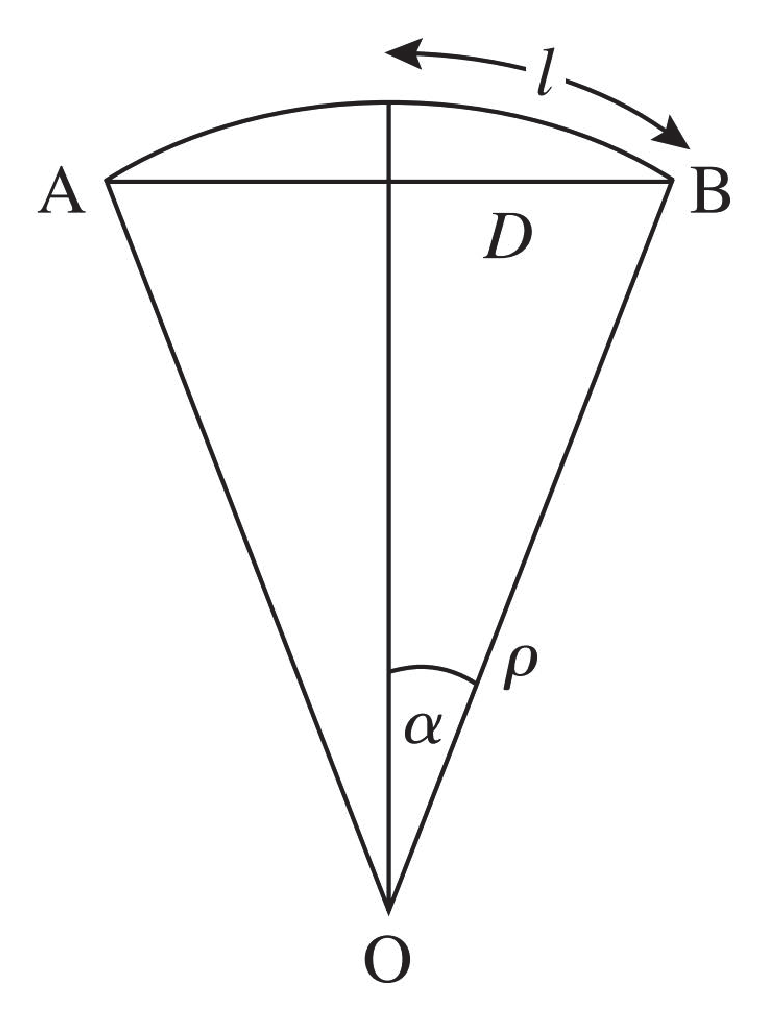
\includegraphics[height=6.cm,angle=0]{2D_analogy.eps}
\caption{} 
\label{fig:2D_analogy}
\end{figure}
%===========================================================================================================================



\cite{2010宇宙大尺度结构的形成, 2012宇宙大尺度结构的形成} \textcolor{red}{原时间隔}:$\dif \tau$
\begin{equation}
\dif \tau^2 = \dif t^2 -R^2(t)\left\lbrace \frac{\dif r^2}{1-kr^2} +r^2 \dif \theta^2 +r^2 \sin^2 \theta \dif \phi^2 \right\rbrace
\end{equation}
取光速为$c = 1$;

写成用度规表示的形式
\begin{equation}
\dif \tau^2 = -g_{\mu \nu} \dif x^{\mu} \dif x^{\nu} = -\sum_{\mu, \nu = 0}^3 g_{\mu \nu} \dif x^{\mu} \dif x^{\nu}
\end{equation}
$x^0 = t$,$x^1 = r$,$x^2 = \theta$,$x^3 = \phi$,

\textcolor{red}{度规张量}:$g_{\mu \nu}$,Robertson—Walker度规(R-W度规);
\begin{eqnarray}
\nonumber g_{00} &=& -1, \\
\nonumber g_{rr} &=& \frac{a^2(t)}{1-kr^2}, \\
\nonumber g_{\theta \theta} &=& a^2(t) r^2, \\
g_{\phi\phi} &=& a^2(t) r^2 \sin^2(\theta), 
\end{eqnarray}
$g_{\mu \nu}$:协变张量,

$g^{\mu \nu}$:逆变张量,

$g_{\mu \alpha} g^{\mu \beta} = \delta^{\alpha}_{\beta}$,

$\delta^{\alpha}_{\beta} = \delta_{\alpha\beta}$:Kronecker delta符号,当$\alpha = \beta$时,$\delta_{\alpha\beta} = 1$,当$\alpha \neq \beta$时,$\delta_{\alpha\beta} = 0$

$g^{\mu \nu}$的分量
\begin{eqnarray}
\nonumber g^{00} &=& -1, \\
\nonumber g^{rr} &=& \frac{1-kr^2}{a^2(t)}, \\
\nonumber g^{\theta \theta} &=& \frac{1}{a^2(t) r^2}, \\
g^{\phi\phi} &=& \frac{1}{a^2(t) r^2 \sin^2(\theta)}, 
\end{eqnarray}

由R --- W度规,超球面$r$与$r+\dif r$之间所包含的\textcolor{red}{固有体积}


$r, \theta, \phi$:\textcolor{red}{共动坐标};球面上每一点的共动坐标是不变的;

$a(t) r$:\textcolor{red}{物理坐标};

在每一个坐标点处再放置一只钟记录宇宙时间,根据宇宙学原理,各处的宇宙时是相同的;对于一个静止于共动坐标系的观测者来说,其世界线是$r, \theta, \phi$为常值的线(\textcolor{red}{测地线});

\textcolor{red}{line element}: isotropic and homogeneous three-dimensional hyper-surface;

\begin{equation}
\dif l^2 = a^2(t)\left\lbrace \frac{\dif r^2}{1-kr^2} +r^2 (\dif \theta^2 + \sin^2 \theta \dif \phi^2) \right\rbrace
\end{equation}

$a(t)$: time-dependent scale factor; relates the coordinate labels $(r,\theta,\phi)$ of the fundamental observers to true physical distance.

\textcolor{red}{proper time} of an observer: the one recorded by the clock at rest with the observer.

\textcolor{red}{cosmic time} $t$: the proper time of all fundamental observers.


\cite{2015eaci.book.....S} 


\cite{perkins2008particle} The actual radius of the visible universe --- the distance to the optical horizon --- is about a factor $3.3$ times larger than the \textcolor{red}{Hubble length $c t_0$}, where is $t_0 = 14$ Gyr. 

The (negative) \textcolor{yellow}{gravitational potential energy $GM^2/R$} and the \textcolor{yellow}{mass energy $Mc^2$ of the universe} are \textcolor{yellow}{comparable} at \textcolor{yellow}{$\sim 10^{70}$ J}, so that the total energy could be quite small. The measured value of curvature parameter on very large scales is consistent with it, and the total energy, being exactly zero. Of the various arbitrary numbers which are needed to describe our universe, this zero value seems to be the only natural one!

\section{Friedmann方程}
\cite{2010宇宙大尺度结构的形成, 2012宇宙大尺度结构的形成} 膨胀宇宙的动力学性质取决于$a(t)$;

\textcolor{red}{爱因斯坦场方程}
\begin{equation}
R_{\mu\nu} = 8\pi G S_{\mu\nu}
\end{equation}
$R_{\mu\nu}$:\textcolor{red}{Ricci张量},
\begin{equation}
R_{\mu\nu} = \frac{\partial \Gamma_{\mu\nu}^{\lambda}}{\partial x^{\lambda}} -\frac{\partial \Gamma_{\mu\lambda}^{\lambda}}{\partial x^{\nu}} +\Gamma_{\mu\nu}^{\delta}\Gamma_{\lambda\delta}^{\lambda} -\Gamma_{\mu\lambda}^{\delta}\Gamma_{\nu\delta}^{\lambda}
\end{equation}
$\Gamma_{\nu\beta}^{\mu}$:\textcolor{red}{仿射联络},
\begin{equation}
\Gamma_{\nu\beta}^{\mu} = \frac{1}{2} g^{\mu\lambda} \left[\frac{\partial g_{\lambda \nu}}{\partial x^{\beta}} +\frac{\partial g_{\lambda\beta}}{\partial x^{\nu}} -\frac{\partial g_{\nu\beta}}{\partial x^{\lambda}} \right]
\end{equation}
$S_{\mu\nu}$:场源项,
\begin{equation}
S_{\mu\nu} = T_{\mu\nu} -\frac{1}{2}g_{\mu\nu} T
\end{equation}
$T_{\mu\nu}$:\textcolor{red}{能量—动量张量},
\begin{equation}
T_{\mu\nu} = (\rho +p) u_{\mu}u_{\nu} +g_{\mu\nu} p
\end{equation}
$\rho$,$p$:宇宙物质的能量密度和压力,

$u_{\mu}$:物质(视为流体)的四维速度,且有$u^0 = u^t = 1$,$u^i = 0~ (i = 1,2,3 \Leftrightarrow i =r, \theta, \phi)$,

$T$:\textcolor{red}{能量—动量张量$T_{\mu\nu}$的迹},
\begin{equation}
T \equiv T^{\mu}_{\mu} = g^{\mu\lambda} T_{\mu\lambda}
\end{equation}




\cite{perkins2008particle} The `Standard Model' of present day cosmology is the solution proposed by Friedmann-Lemaitre-Robertson-Walker (FLRW for short), which assumes a completely isotropic and homogenous distribution of matter and radiation, behaving like a perfect frictionless fluid. Even today the average separation between galaxies is of order 100 times their diameter and the overall expansion of the universe of billions of galaxies on large enough scales, that is many orders of magnitude larger than the intergalactic separations, still appears to be reasonably well described by the FLRW model. The time components of the field equations is
\begin{equation} 
\color{red} H^2 = \left(\dfrac{\dot{R}}{R} \right)^2 = \dfrac{8\pi G \rho_{\rm tot}}{3} - \dfrac{kc^2}{R^2} ~,
\label{eq:Friedmann_time}
\end{equation}
where $R = R(t)$ is the expansion parameter, $\rho_{\rm tot}$ is the total density of matter, radiation, and vacuum energy, as described below, and $G$ is Newton's gravitational constant. This equation follows when the FLRW metric is inserted in the Einstein field equations. \textcolor{red}{$kc^2/R^2$} is the \textcolor{red}{curvature term}. In the presence of gravitating masses, the `flat' Euclidean space of special relativity is replaced by curved space/time. \textcolor{blue}{A light beam going from point A to point B will travel along a path which is an extremum}, which is the \textcolor{blue}{shortest spatial path length} (and also the \textcolor{blue}{path of maximum proper time}) called a \textcolor{red}{geodesic}. Geodesics are straight lines in Euclidean space, but in the presence of gravitational fields, the paths are curved. 

In the language of particle physics, one might say that \textcolor{yellow}{space/time appears curved because photons are deflected (and also retarded) by gravitational fields, mediated by graviton exchange}. The curvature parameter $k$ can assume values of $+1$, $0$, or $-1$, corresponding to the curvature $k/R^2$ being positive, zero, or negative respectively. The two-dimensional analogy for positive or convex curvature is the surface of a sphere, while that for negative or concave curvature is as in a saddle.

Consider a point mass $m$ being accelerated by gravity at the surface of a sphere of radius $D$, density $\rho$, and mass $M = 4\pi D^3 \rho/3$. According to Newtonian mechanics, the assumed spherically symmetric and homogeneous distribution of matter outside of the sphere can make no contribution to the force, while the field at the surface is the same as if all the mass were concentrated at the centre. This is also true in general relativity (by a theorem due to Birkhoff). The force equation is
\begin{equation}
m \ddot{D} = -\dfrac{mMG}{D^2} ~,
\label{eq:Newtonian}
\end{equation}
Express $M$ in terms of $D$ and $\rho$, factors of $r$ from $D(t) = r \cdot R(t)$ cancel out.
\begin{empheq}[box=\widefbox]{align*}
& \dfrac{\dif \dot{D}}{\dif D} \dfrac{\dif D}{\dif t} = - \dfrac{mMG}{D^2} \\
& \dot{D} \dif \dot{D} = - \dfrac{mMG}{D^2} \dif D \\
& \dfrac{\dot{D}^2}{2} = \dfrac{mMG}{D} + \rm constant \\
& \dfrac{\dot{R}^2}{2} -\dfrac{MG}{R} = \rm constant 
\end{empheq}
\begin{align}
\dfrac{m\dot{R}^2}{2} - \dfrac{mMG}{R} = {\rm constant} = -\dfrac{mkc^2}{2} ~.
\end{align}
If multiplying through by $2/mR^2$, we obtain an equation in agreement with (\ref{eq:Friedmann_time}), after setting the constant of integration equal to the value given by general relativity. The terms on the left-hand side correspond to the kinetic and potential energies of the mass $m$, and so the so-called curvature term on the right simply represents the total energy. $k = -1$ corresponds to \textcolor{blue}{negative curvature and positive energy}, that is to say an \textcolor{blue}{open universe expanding without limit}. For $k = -1$, $\dot{R}(t) = r \cdot \dot{R}(t) \rightarrow c$ at large enough values of $R$. A value $k = +1$ corresponds to \textcolor{blue}{a closed universe with negative total energy and positive curvature}, which reaches a maximum radius and then collapses. $k = 0$ is the simplest case, where the \textcolor{blue}{kinetic and potential energies just balance} and the \textcolor{blue}{total energy and curvature are both zero}. The universe expands forever but the velocity tends asymptotically to zero at large $t$. This case is called the \textcolor{blue}{flat universe}. These three cases are illustrated in Fig. \ref{fig:scalefactor}. 

%===========================================================================================================================
\begin{figure}
\centering
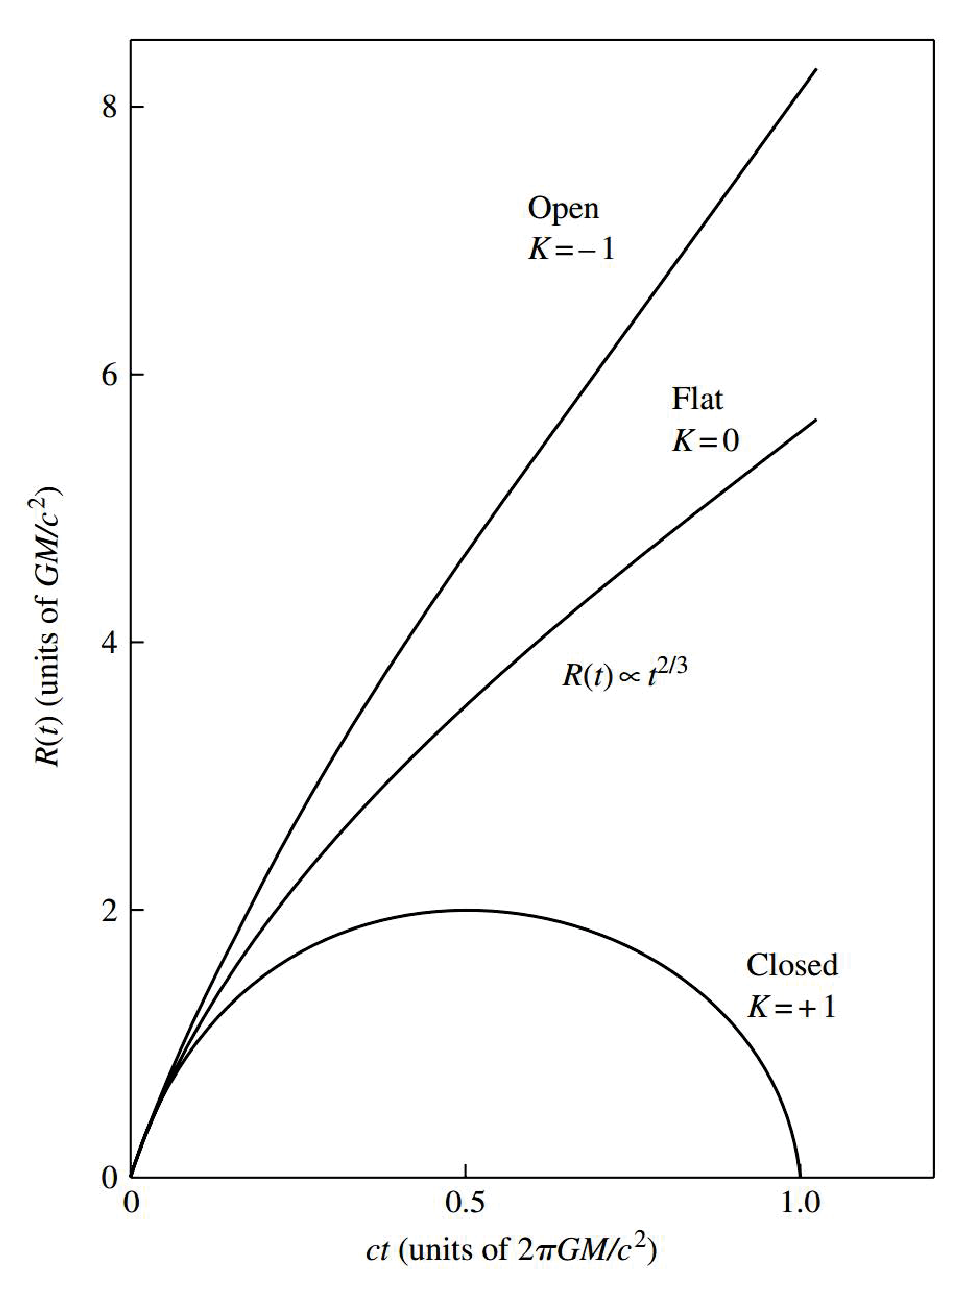
\includegraphics[height=12.cm,angle=0]{scalefactor_evo.eps}
\caption{Dependence of the scale factor $R(t)$ on time for three different $k$ values. At the present time, our universe appears to be extremely close to the $k = 0$ curve. At early times, the parameter $R(t)$ varies as $t^{2/3}$
for all $k$ values. For a vacuum-dominated universe, on the contrary, the scale factor increases exponentially with
time. In the distant past, when the universe was only half its present age, it seems that it was indeed matter dominated. However, at the present time, the contribution to the total energy density from the vacuum is
more than twice that due to matter. The present age of the universe corresponds to the very early part of the $k = 0$
curve (roughly $0.15$ on the $x$-axis scale).} 
\label{fig:scalefactor}
\end{figure}
%===========================================================================================================================

For the case $k = 0$ and a universe dominated by non-relativistic matter of conserved mass $M$,
\begin{empheq}[box=\widefbox]{align*}
\left(\dfrac{\dot{R}}{R} \right)^2 &= \dfrac{2GM}{R^3} \\
\dot{R}^2 &= \dfrac{2GM}{R} \\
\sqrt{R} \dot{R} &= \sqrt{2GM} \\
R^{1/2} \dif R &= \sqrt{2GM} \dif t \\
\dfrac{2}{3} \dif R^{3/2} &= \sqrt{2GM} \dif t \\
R^{3/2} &= \left(\dfrac{9GM}{2}\right)^{1/2} t \\
R(t) &= \left(\dfrac{9GM}{2}\right)^{1/3} t^{2/3} 
\end{empheq}
\begin{equation}
R(t) = \left(\dfrac{9GM}{2} \right)^{1/3} t^{2/3} ~,
\end{equation}
the \textcolor{red}{Hubble time} is $1/H_0 = R(0)/\dot{R}(0) = 3t_0/2$ and the age of the universe is 
\begin{equation}
t_0 = \dfrac{2}{3H_0} = 9.1\pm 0.2 ~\rm Gyr ~.
\end{equation}
Other estimates of the age of the universe give significantly larger values. They come, for example, from study of the \textcolor{blue}{luminosity-colour relation} (Herzsprung-Russell diagram) in the \textcolor{blue}{oldest star populations}, the \textcolor{blue}{globular clusters}; from \textcolor{blue}{cooling rates of white dwarf stars}; and from dating using \textcolor{blue}{isotopic ratios of radioactive elements in the Earth's crust} and in \textcolor{blue}{very old stars}. All these estimates straddle an approximate range for the age of the universe of
\begin{equation}
t_0 = 14 \pm 1 ~{\rm Gyr} ~.
\end{equation}

Example: Show that for a curvature term with $k = +1$, the Big Bang would be followed by a Big Crunch at time $t = 2 \pi GM /c^3$ where $M$ is the (assumed conserved) mass of the universe.

For $k = +1$, the Friedmann equation becomes $\left(\dfrac{\dot{R}}{R} \right)^2 = \dfrac{2GM}{R^3} -\dfrac{c^2}{R^2}$. $\dot{R} = 0$ when $R = \dfrac{2GM}{c^2}$, which is the maximum radius. The element of time is then given by $\dif t = \dfrac{\dif R}{\left(\dfrac{2GM}{R} - c^2 \right)^{1/2}}$. Substituting $\dfrac{2GM}{R}-c^2 = c^2 \tan^2 \theta$ the total time to the maximum is $\dfrac{4GM}{c^3} \int \cos 2\theta \dif \theta = \dfrac{\pi GM}{c^3}$. By symmetry the time to the subsequent crunch is just twice this. $M = 10^{23} M_\odot$ gives $t \sim 100$ Gyr. 
\begin{empheq}[box=\widefbox]{align*}
& \left(\dfrac{\dot{R}}{R} \right)^2 = \dfrac{8\pi G \rho_{\rm tot}}{3} - \dfrac{kc^2}{R^2} \\
& \left(\dfrac{\dot{R}}{R} \right)^2 = \dfrac{2GM}{R^3} -\dfrac{c^2}{R^2} \\
& \dot{R}^2 = \dfrac{2GM}{R} -c^2 \\
& \dfrac{R^{1/2}}{\sqrt{2GM}} \dot{R} = \sqrt{1 -\dfrac{c^2 R}{2GM} } \\
& \dfrac{R^{1/2}}{ \sqrt{1 -\dfrac{c^2 R}{2GM} }} \dif R = \sqrt{2GM} \dif t \\
& -\dfrac{2GM}{c^2} \dfrac{R^{1/2}}{ \sqrt{1 -\dfrac{c^2 R}{2GM} }}  \dif \left( 1-\dfrac{c^2 R}{2GM} \right)  = \sqrt{2GM} \dif t \\
& \int -2\dfrac{\sqrt{2GM} }{c^2} R^{1/2}  \dif \sqrt{1 -\dfrac{c^2 R}{2GM} }  = t \\
& -2\dfrac{\sqrt{2GM} }{c^2} \left( R^{1/2} \sqrt{1 -\dfrac{c^2 R}{2GM} } -\int \sqrt{1 -\dfrac{c^2 R}{2GM} } \dif R^{1/2} \right) = t \\
& t = 2\dfrac{\sqrt{2GM} }{c^2} \int \sqrt{1 -\dfrac{c^2 R}{2GM} } \dif R^{1/2} \\
& t = \dfrac{4GM}{c^3} \int \sqrt{1 -\dfrac{c^2 R}{2GM} } \dif \dfrac{cR^{1/2}}{\sqrt{2GM}} \\
& t = \dfrac{2 \pi GM}{c^3}
\end{empheq}


Example: Find solutions of the Friedmann equation for the case of a matter-dominated universe of total mass $M$, and values of $k = +1$ and $k = -1$.

$$ \left(\dfrac{\dot{R}}{R} \right)^2 = \dfrac{2GM}{R} -kc^2$$
For $k = +1$, the solution for $R$ as a function of $t$ has the parametric form of a cycloid curve (i.e. the curve traced out by a point on the circumference of a circular disc rolling along a plane):
\begin{align*}
R &= a(1-\cos \theta) \\
t &= b(\theta -\sin \theta) ~.
\end{align*}
The constants $a = \dfrac{MG}{kc^2}$ and $b = \dfrac{MG}{(kc^2)^{3/2}}$, and the parameter $\theta$ is the angle of rotation of the cycloid. For $k = -1$,
\begin{align*}
R &= a(\cosh \theta -1) \\
t &= b(\sinh \theta - \theta) ~.
\end{align*}
with the above values of $a$ and $b$, and $k$ replaced by $|k|$. By expanding the above circular functions for small values of $\theta$, for either $k = +1$ or $-1$, the expansion parameter $R \propto t^{2/3}$, that is the same as for the case $k = 0$.
 






























































\section{The sources of energy density}
\cite{2010宇宙大尺度结构的形成, 2012宇宙大尺度结构的形成} 1. 若宇宙仅由物质(包括辐射)组成,在Robertson-Walker度规下,得到$R_{\mu\nu}$不为零的分量:
\begin{eqnarray}
R_{00} &=& -3\frac{\ddot{a}}{a}, \\
R_{ij}   &=& [a\ddot{a} +2\dot{a}^2 +2k] \tilde{g}_{ij}
\end{eqnarray}
$k = 0, \pm 1$,

$\tilde{g}_{ij}~ (i, j = r, \theta, \phi)$:纯空间度规,其不为零的分量:
\begin{eqnarray}
\nonumber \tilde{g}_{rr} &=& \frac{1}{1-kr^2}, \\
\nonumber \tilde{g}_{\theta\theta} &=& r^2, \\
\tilde{g}_{\phi\phi} &=& r^2 \sin^2 \theta
\end{eqnarray}
且
\begin{equation}
g_{ij} = a^2(t) \tilde{g}_{ij}
\end{equation}
对能量---动量张量和它的迹
\begin{eqnarray}
\nonumber T_{00} &=& \rho, \\
\nonumber T_{ij} &=& p g_{ij} = pa^2 \tilde{g}_{ij}, \\
T &=& -\rho +3p
\end{eqnarray}
场源项$S_{\mu\nu}$
\begin{eqnarray}
S_{00} &=& T_{00} -\frac{1}{2} g_{00} T = \frac{1}{2}(\rho +3p), \\
S_{ij}  &=& T_{ij} -\frac{1}{2} g_{ij} T = \frac{1}{2}(\rho -p) a^2 \tilde{g}_{ij}
\end{eqnarray}

爱因斯坦场方程的时—时分量
\begin{equation}
\ddot{a} = -\frac{4\pi G}{3} (\rho +3p) a
\label{tt_comp}
\end{equation}
空—空分量
\begin{equation}
[a\ddot{a} + 2\dot{a}^2 +2k] \tilde{g}_{ij} = 8\pi G\left[p +\frac{1}{2}(\rho -3p) \right] a^2 \tilde{g}_{ij}
\end{equation}
即
\begin{equation}
a\ddot{a} + 2\dot{a}^2 +2k = 4\pi G(\rho -p) a^2
\label{ss_comp1}
\end{equation}
把式(\ref{tt_comp})代入式(\ref{ss_comp1})消去$\ddot{a}$,可得
\begin{equation}
\dot{a}^2 +k = \frac{8\pi G}{3} \rho a^2
\label{ss_comp2}
\end{equation}
式(\ref{tt_comp})和式(\ref{ss_comp2})称为\textcolor{red}{Friedmann方程},是描述宇宙尺度因子$a(t)$演化的基本方程;

2. 若包括真空能量,设物质(或真空能量)的物态方程
\begin{equation}
p = w \rho
\end{equation}
则
\begin{equation}
\rho \propto a^{-3(1+w)}
\end{equation}
冷物质(非相对论性物质,如尘埃)
\begin{equation}
p = 0 \Rightarrow w = 0 \Rightarrow \rho \propto a^{-3}, ~a(t) \propto t^{2/3}
\end{equation}
热物质(相对论性物质,如辐射)
\begin{equation}
p = \rho/3 \Rightarrow w = 1/3 \Rightarrow \rho \propto a^{-4}, ~a(t) \propto t^{1/2}
\end{equation}
真空能量,宇宙学常数
\begin{equation}
p = -\rho \Rightarrow w = -1 \Rightarrow \rho \equiv \rho_V = \text{常量}, ~a(t) \propto \exp(Ht), H = \sqrt{\frac{8\pi G\rho_V}{3}}
\end{equation}
\textcolor{red}{宇宙学常数}
\begin{equation}
\Lambda = 8\pi G\rho_V
\end{equation}


\cite{perkins2008particle} The conservation of energy $E$ in a volume element $\dif V$ of our perfect cosmic fluid can be expressed as
\begin{equation}
\dif E = -P \dif V ~,
\end{equation}
where $P$ is the pressure. With $\rho c^2$ as the energy density this becomes
\begin{align}
\nonumber & \dif (\rho c^2 R^3 ) = -P \dif R^3 \\
& \dot{\rho} = -3 \left( \dfrac{\dot{R}}{Rc^2} \right) \left( P + \rho c^2 \right) ~.
\label{eq:rho_diff}
\end{align}
\begin{empheq}[box=\widefbox]{align*}
& \left(\dfrac{\dot{R}}{R} \right)^2 = \dfrac{8\pi G \rho}{3} - \dfrac{kc^2}{R^2} \\
& 2  \dfrac{\dot{R}}{R} \cdot  \dfrac{(\ddot{R}R -\dot{R}^2)}{R^2} = \dfrac{8\pi G}{3} \dot{\rho} - (-2) \dfrac{kc^2}{R^3} \dot{R} \\
&2  \dfrac{\dot{R}}{R} \cdot \left( \dfrac{\ddot{R}}{R} - H^2\right) = \dfrac{8\pi G}{3} (-3) \left( \dfrac{\dot{R}}{Rc^2} \right) \left( P + \rho c^2 \right) + 2\dfrac{kc^2}{R^3} \dot{R} \\
& \dfrac{\ddot{R}}{R} - \left( \dfrac{8\pi G \rho}{3} - \dfrac{kc^2}{R^2} \right) = - \dfrac{4\pi G}{3} \left( \dfrac{3P}{c^2} + 3\rho \right) +\dfrac{kc^2}{R^2} \\
& \dfrac{\ddot{R}}{R} = - \dfrac{4\pi G}{3} \left( \dfrac{3P}{c^2} + \rho \right) 
\end{empheq}
\begin{equation}
\ddot{R} = - \dfrac{4\pi G R}{3} \left( \dfrac{3P}{c^2} + \rho \right) 
\end{equation}
which is the same as (\ref{eq:Newtonian}) for the case $P \approx 0$ for non-relativistic matter. $\rho$ and $P$ will be connected by an equation of state, 
\begin{equation}
\color{red} P = w \rho c^2 ~,
\label{eq:eofs}
\end{equation}
where $w$ is a parameter which may be constant, as it is for matter, radiation, and the vacuum state, or might be time dependent. If $w$ is in fact time independent, from (\ref{eq:rho_diff}) and (\ref{eq:eofs}),
\begin{equation}
\color{red} \rho \propto R^{-3(1+w)} ~.
\end{equation}
The variation of $\rho$ with $R$ follows for the different regimes shown in Fig. \ref{fig:rho_R_evo}.

%===========================================================================================================================
\begin{figure}
\centering
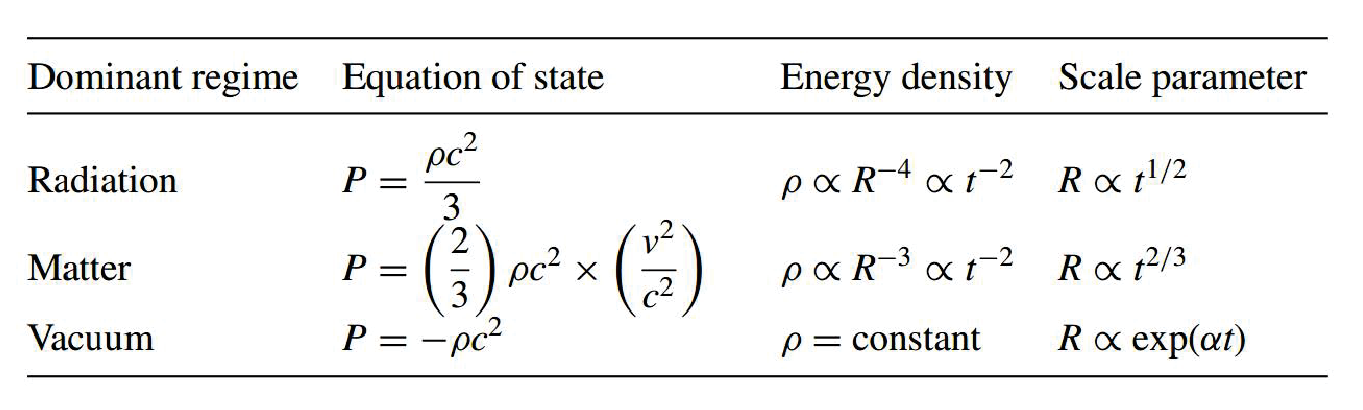
\includegraphics[height=4.cm,angle=0]{rho_R_evo.eps}
\caption{Energy density and scale parameters for different regimes} 
\label{fig:rho_R_evo}
\end{figure}
%===========================================================================================================================

The overall density $\rho$ in the Friedmann equation is generally considered to  be made up of (at least) three components, corresponding to the contributions from matter, radiation, and the vacuum state:
\begin{equation}
\color{blue} \rho_{\rm tot} = \rho_{m} +\rho_r +\rho_\Lambda ~.
\end{equation}
$\rho_\Lambda$, which we have here identified with the \textcolor{blue}{vacuum state}, can be incorporated in the Friedmann equation as a \textcolor{red}{cosmological constant $\Lambda$},
\begin{equation}
\rho_\Lambda = \dfrac{\Lambda}{8\pi G} ~.
\end{equation}
If a term $\Lambda/3$ is added to the right-hand side of (\ref{eq:Friedmann_time}), then at large enough $R(t)$ this term will dominate and the expansion will become exponential, that is, $R(t) \propto \exp(\alpha t)$ where $\alpha = (\Lambda/3)^{1/2}$.


Suppose we have an ideal gas consisting of particles of mass $m$, velocity $v$, and momentum $mv$, confined within a cubical box of side $L$ with walls with which the particle collides elastically (see Fig. \ref{fig:equations_of_state}a). A particle with $x$-component of velocity $v_x$ will strike a particular face normal to the $x$-axis at a rate of $v_x/2L$ collisions per unit time. As the component of momentum $p_x = mv_x$ is reversed at each collision, the rate of change of momentum and therefore the force exerted by the particle will be $2mv_x \cdot (v_x/2L)$. The pressure exerted by the particle on the face of the box, which has area $A = L^2$, is $mv_x^2/L^3$, where $V = L^3$ is the volume. If there are $n$ particles per unit volume, it follows that the pressure they exert will be $mnv_x^2$ where $v_x^2$ is a mean square value. Since the gas is isotropic, the mean square values of the $x$, $y$, and $z$ components of velocity will be equal and the pressure will be
\begin{equation}
P = \left( \dfrac{1}{3} \right) mn \left\langle v^2 \right\rangle = \left( \dfrac{1}{3} \right) n \left\langle p v \right\rangle
\end{equation}
Assume that the gas consists of non-relativistic particles. The values of the kinetic energy density $\epsilon$ and of the pressure are
\begin{align}
& \epsilon = \left( \dfrac{1}{2} \right) mn \left\langle v^2 \right\rangle \\
& P_{\rm non-rel} = \left( \dfrac{2}{3} \right) \epsilon = \left( \dfrac{2}{3} \right) \rho c^2 \times  \left( \dfrac{v^2}{c^2} \right)
\end{align}
where $\rho c^2$ is the total energy density of matter, including the mass energy. Since for cosmic matter in general, $v^2 \ll c^2$, the pressure it exerts is very small.

If the gas particles have extreme relativistic velocities, the energy density and the pressure, usually called the radiation pressure, 
\begin{align}
& \rho c^2 =  mn  c^2  \\
& P_{\rm rel} = \dfrac{\rho c^2}{3} 
\end{align}

%===========================================================================================================================
\begin{figure}
\centering
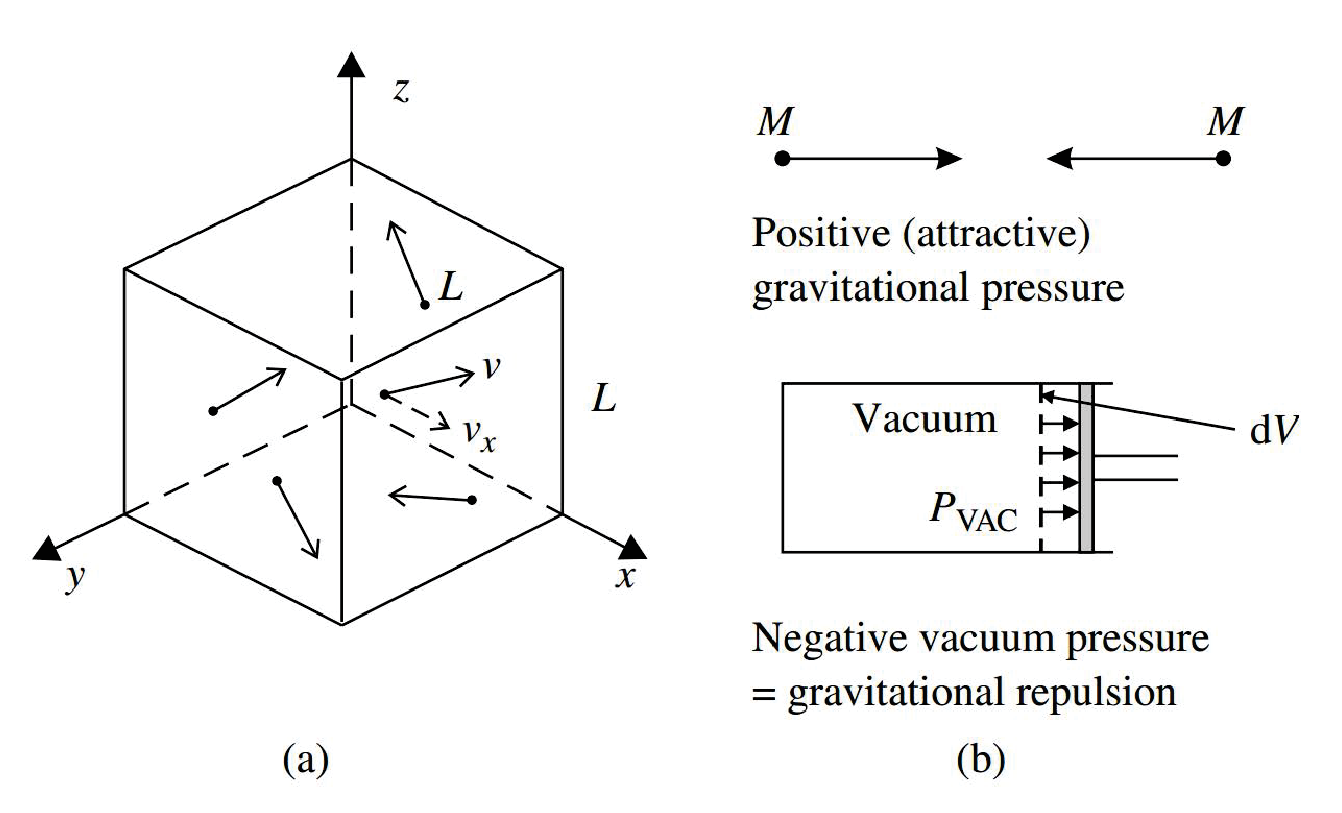
\includegraphics[height=8.cm,angle=0]{equations_of_state.eps}
\caption{} 
\label{fig:equations_of_state}
\end{figure}
%===========================================================================================================================

The vacuum may contain an energy density and exert a pressure equivalent to a gravitational repulsion may seem strange, since in classical physics, a vacuum is supposed to contain absolutely nothing. However, in quantum field theory, as has been discussed for the electroweak model the Uncertainty Principle actually requires that the vacuum contains virtual particle-antiparticle pairs which spontaneously appear and disappear, and the vacuum itself is defined, not as nothing but as the state of \textcolor{blue}{lowest possible energy of the system}. Because the virtual particles carry energy and momentum, if only on a temporary basis, general relativity implies that they must be coupled to gravitation. Indeed, the measurable effect of such vacuum energy is through its gravitational influence.

The relation \textcolor{blue}{$P = -\rho c^2$} for this \textcolor{blue}{lowest energy vacuum state} can be formally shown to follow from \textcolor{blue}{Lorentz invariance}, that is, the requirement that the \textcolor{blue}{state must look the same to all observers}, implying also that the \textcolor{blue}{energy density must have the same constant value everywhere and for all time}. Assume that we have a piston enclosing an isolated cylinder filled with the vacuum state of energy density $\rho c^2$. If the piston is withdrawn adiabatically by an element of volume $\dif V$, the extra vacuum energy created will be $\rho c^2 \dif V$, and this must be supplied by the work done by the vacuum pressure, $P \dif V$. Hence by energy conservation $P = -\rho c^2$ and from (\ref{eq:rho_diff}), $\rho =$ constant.

\section{Observed energy densities}
\textcolor{red}{宇宙临界密度}
\begin{equation}
\rho_c \equiv \frac{3H_0^2}{8\pi G} = 1.88 \times 10^{-29} h^2~ \text{g}/\text{cm}^3 = 2.78 \times 10^{11} h^2 ~ M_{\odot}/\text{Mpc}^3
\end{equation}

\cite{perkins2008particle} For $k = 0$, (\ref{eq:Friedmann_time}) gives a value for the \textcolor{red}{critical density} which (today) would just close the universe
\begin{align}
& \rho_c = \dfrac{3}{8\pi G} H_0^2 = 9.6 \times 10^{-27} ~{\rm kg ~m^{-3}} \\
& \rho_c c^2 = 5.4 \pm 0.5 ~ {\rm GeV ~m^{-3}}
\end{align}
The \textcolor{green}{ratio of the actual density to the critical density} is called the \textcolor{red}{closure parameter}, which at the present time and for arbitrary $k$ is
\begin{empheq}[box=\widefbox]{align*}
& H^2 = \dfrac{8\pi G}{3} \rho - \dfrac{kc^2}{R^2} \\
& H_0^2 = \dfrac{8\pi G}{3} \rho_c \\
& \dfrac{H^2}{H_0^2} = \dfrac{\rho}{\rho_c} -\dfrac{kc^2}{[H_0R(0) ]^2} \\
& \dfrac{\rho}{\rho_c} = 1 +\dfrac{kc^2}{[H_0R(0)]^2}
\end{empheq}
\begin{equation}
\color{blue} \Omega = \dfrac{\rho}{\rho_c} = 1 + \dfrac{kc^2}{[H_0 R(0)]^2}
\end{equation}
A flat universe with $k = 0$ will have $\Omega = 1$ for all values of $t$. The different contributions to the total value of $\Omega$ are, 
\begin{equation}
\color{blue} \Omega = \Omega_r +\Omega_m +\Omega_\Lambda ~.
\end{equation}
If $k \neq 0$, one can express the curvature term as
\begin{equation}
\color{red} \Omega_k = \dfrac{\rho_k}{\rho_c} = - \dfrac{kc^2}{[H_0 R(0)]^2} ~,
\end{equation}
\begin{equation}
\color{blue} \Omega  + \Omega_k = \Omega_r +\Omega_m +\Omega_\Lambda +\Omega_k = 1 ~.
\end{equation}
At the present time, the density of the microwave photon radiation corresponds to $\Omega_r = 5 \times 10^{-5}$, and is completely negligible in comparison with that of matter, while the vacuum term $\Omega_\Lambda$ makes a major contribution. In addition to the microwave photon relics of the Big Bang, there are relic neutrinos and antineutrinos, with comparable number density and quantum energy to the photons. Because these \textcolor{orange}{neutrinos have masses comparable with or larger than their kinetic energies today}, they are \textcolor{orange}{non-relativistic}. However, at early times in the universe when it was much hotter and radiation-dominated, they were extreme relativistic and so would be included in the radiation term, increasing the radiation energy density by some \textcolor{yellow}{$58 \%$}.

Apart from a very small energy density contribution in microwave photons and neutrinos, the energy density of the universe today is made up of several components as follows:
1. For luminous baryonic matter (i.e. visible protons, neutrons, and nuclei) in the form of stars, gas, and dust it is found that
\begin{align}
& \rho_{\rm lum} = 9 \times 10^{-29} ~{\rm kg ~m^{-3}} \\
& \Omega_{\rm lum} = 0.01
\end{align}
2. The total density of baryons, visible or invisible, as inferred from the model of nucleosynthesis, is about $0.26$ baryons $m^{-3}$, or an energy density
\begin{align}
& \rho_{b} = 4 \times 10^{-28} ~{\rm kg ~m^{-3}} \\
& \Omega_{b} = 0.042 \pm 0.004
\end{align}
3. The total matter density, as inferred from the gravitational potential energy deduced from galactic rotation curves  and the kinematics of large-scale structures in the universe is
\begin{align}
& \rho_{m} = 2.2 \times 10^{-27} ~{\rm kg ~m^{-3}} \\
& \Omega_{b} = 0.24 \pm 0.003
\end{align}
4. The dark (or vacuum) energy density can be measured from an observed curvature in the Hubble plot, obtained from study of Type 1A supernovae at large redshifts. It may also be inferred from the position of the `acoustic peaks' in the angular power spectrum of the temperature fluctuations in the microwave radiation measuring the total density
\begin{equation}
\Omega_{\rm tot} = 1.0 \pm 0.02
\end{equation}
which indicate a value for the dark energy density of
\begin{equation}
\Omega_\Lambda = 0.76 \pm 0.05 ~.
\end{equation}
$H_0$ is specified as $100 h$ km s$^{-1}$ Mpc$^{-1}$ where $h = 0.72$. In that case the critical density would be quoted as $\rho_c/h^2$ and the value of the closure parameter as $\Omega h^2$, where $h^2 = 0.52$. 





















\section{The deceleration parameter: the effects of vacuum energy/cosmological constant}
\cite{perkins2008particle} The time dependence of the expansion parameter as a Taylor series is
\begin{align}
\nonumber & R(t) = R(0) + \dot{R}(0) (t-t_0) + \left(\dfrac{1}{2} \right) \ddot{R}(0)(t-t_0)^2 + \cdots \\
\nonumber & \dfrac{R(t)}{R(0)} = 1+H_0(t-t_0) - \left(\dfrac{1}{2} \right) q_0 H_0^2 (t-t_0)^2 +\cdots
\end{align}
where the \textcolor{red}{deceleration parameter}, which can be \textcolor{blue}{time dependent}, is defined as
\begin{align}
q &= \color{yellow}  -\dfrac{\ddot{R} R}{{\dot{R}}^2} \\
&= \left[\dfrac{4\pi G}{3c^2 H^2} \right] [\rho c^2 +3 P] \\
&= \color{yellow} \dfrac{\Omega_m}{2} +\Omega_r -\Omega_\Lambda ~.
\end{align}
\begin{empheq}[box=\widefbox]{align*}
\ddot{R} &= - \left(\dfrac{4\pi GR}{3}  \right)  \left(\rho +\dfrac{3P}{c^2}  \right) \\
\dfrac{\ddot{R} R}{\dot{R}^2} &= - \left(\dfrac{4\pi GR^2}{3 \dot{R}^2 }  \right)  \left(\rho +\dfrac{3P}{c^2}  \right) \\
- \dfrac{\ddot{R} R}{\dot{R}^2} &= \left(\dfrac{4\pi G}{3 c^2 H^2 }  \right)  \left(\rho c^2 +3P  \right) 
\end{empheq}
Today $\Omega_m \gg \Omega_r$, so that if $\Omega_\Lambda$ could be neglected, a flat universe would have $\Omega = \Omega_m = 1$ and $q = 0.5$, that is, the universal expansion must be decelerating because of the retarding effects of the gravitational attraction of matter. In fact, early attempts to measure $q$ seemed to give results consistent with this value (within large errors). We may note that if $\Omega_\Lambda$ is large enough however, $q < 0$ and the expansion would be accelerating, the vacuum energy having the same effect as a gravitational repulsion. As mentioned above, surveys on Type 1A supernovae at high redshifts, treating them as `standard candles', appear to indicate that $q$ is negative. These surveys show that several billion years ago, that is, for redshifts $z > 1$, the universe was indeed decelerating, but that more recently this deceleration has been replaced by an acceleration. We note that an empty universe, that is one with $\Omega_m = \Omega_\Lambda = \Omega_r = 0$, and hence $\Omega_k = 1$, is neither accelerating nor decelerating, with $H$ independent of time.




\cite{2010宇宙大尺度结构的形成, 2012宇宙大尺度结构的形成}  \textcolor{red}{减速参数(减速因子)$q_0$}:
\begin{equation}
q_0 = -\frac{\ddot{a}(t_0) a(t_0)}{\dot{a}^2(t_0)}
\end{equation}





















%%%%%%%%%%%%%%%%%%%%%%%%%%%%%%%%%%%%%%%%%%%%%%%%%%%%%%%%%%%%%%%%%%%%%%
\bibliographystyle{unsrt_update}
\bibliography{ref}
%%%%%%%%%%%%%%%%%%%%%%%%%%%%%%%%%%%%%%%%%%%%%%%%%%%%%%%%%%%%%%%%%%%%%%


\end{document}
